\documentclass[12pt]{article}
\usepackage{fancyhdr}
\usepackage{amsmath}
\usepackage{fancyvrb}
\usepackage{tikz}
\usepackage{caption}
\usepackage{amsthm}
\usepackage{booktabs}
\usepackage{wrapfig}
\usepackage{algorithm}% http://ctan.org/pkg/algorithms
\usepackage{algpseudocode}% http://ctan.org/pkg/algorithmicx
\usepackage{xcolor}
\usepackage[colorlinks = true,
            linkcolor = blue,
            urlcolor  = blue,
            citecolor = blue,
            anchorcolor = blue]{hyperref}
\usepackage{wrapfig, blindtext}
\usepackage{lipsum}
\usepackage{setspace}
\usepackage{enumitem}
\usepackage[utf8]{inputenc}
\usepackage{tcolorbox}
\usepackage [english]{babel}
\usepackage [autostyle, english = american]{csquotes}
\MakeOuterQuote{"}
\usepackage{listings}
\usepackage{amssymb}
\usepackage[a4paper, left=1.5cm, right=1.5cm, top=2.5cm, bottom=1.5cm]{geometry}
\renewcommand{\thesection}{\Roman{section}} 
\renewcommand{\thesubsection}{\thesection.\Roman{subsection}}
\usepackage{titlesec}
\titleformat*{\section}{\fontsize{12}{5}\selectfont}
\titleformat*{\subsection}{\fontsize{12}{5}\selectfont}
\titlelabel{\thetitle.\enspace}
\usepackage{etoolbox}
\patchcmd{\thebibliography}{\section*}{\section}{}{}
\usepackage{fancyvrb}
\usepackage{gensymb}
\usepackage{pgfplots}
\pgfplotsset{compat=1.11}
\pagestyle{fancy}
\fancyhead{}
\fancyfoot{}
\fancyhead[L]{Evolutionary Time and Protein-Protein Interaction Networks}
\fancyhead[R]{STA 596}
\fancyfoot[C]{\thepage}
\usepackage{graphicx}
\usepackage{hyperref}
\usepackage{xcolor}

\usepackage{indentfirst}

\begin{document}
\title{\textbf{Evolutionary Time and Protein-Protein Interaction Networks}}
\author{Research Paper \\ \\ STA 596: Practical Data Science \\ Jesse Hautala \\ Shawn Houser \\ Angyalka Valcsics }

	\maketitle
\onehalfspacing

\noindent Contents
\begin{enumerate}[label = \Roman{*}.]
\item Introduction
\item Background
\item Methods
\item Results
\item Conclusion
\item Appendix
\item References \newline
\end{enumerate}

\section{Introduction}
Proteins control all biological systems in a cell and, through various interactions with each other, enable cells to complete tasks such as: enzyme activation, gene regulation, and intercellular communication. A system of proteins can be modeled by an undirected network of protein-protein interactions (a PPI network, or PPIN), with nodes representing proteins and edges representing interactions (see Figure 1). The complete set of such interactions for a species is called the protein interactome. When interaction relationships between proteins break, possibly due to environmental factors or random mutations, such breakage can cause disease and death, of the cell and of the organism. We hypothesize that the evolutionary time of a species, which is defined as the total branch length from the root to the leaf representing that species in the tree of life, is directly related to network statistics which describe the topological stability of the species’ protein interactome.

\section{Background}
Advances in proteomics allow researchers to study the protein interactome, but limitations of experimental methods in practice prevent PPI networks from being comprehensive and free of noise. We regard extant PPIN data, including the data used in this project, as a noisy sample from the true protein interactome. For example, the yeast-two-hybrid method for mapping protein interactomes was first developed in 1989 by Fields and Song using \textit{Saccharomyces cerevisiae} as a biological model. The accuracy of this experimental method is estimated to be less than 10 percent. Consequently, the population being studied is the true protein interactome for each species and the variables of interest are the network statistics.

Understanding how protein interactomes evolve and developing methods for analyzing PPI networks is a central goal of evolutionary systems biology (Maddamsetti (2021)). In a paper by Rohan Maddamsetti they provided evidence that protein interactomes in E-Coli appear to show a generational increase in network resilience. Marinka Zitnik (Zitnik \textit{et al.} (2019)) defined network resilience as the measure of how quickly a network breaks down as edges between nodes are randomly removed. A resilience rating of 1 implies that the network is most resilient while a rating of 0 implies a complete loss of connectivity in the PPI network. The current research identified a positive linear relationship between the resilience of an interactome and evolutionary time of the species.

\section{Methods}
\subsection{Acquisition of Data}
Our dataset comes from the Stanford Network Analysis Platform (or SNAP). This data was collected using the Search Tool for the Retrieval of Interacting Genes/Proteins (or STRING), from the European Molecular Biology Laboratory, and organized in multiple text files, joined by species ID. It comprises taxonomy information, an edge set for each interactome, and a numerical variable for evolutionary time of the species.

\begin{wrapfigure}{l}[0pt]{0pt}
\centering
  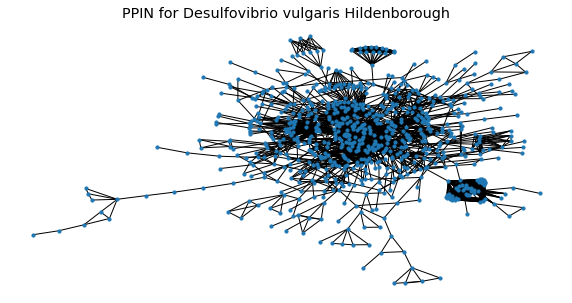
\includegraphics[width=.5\linewidth]{PPIN_fig1}
  \caption{An example PPIN}
  \label{fig:PPIN_fig1}
\end{wrapfigure}

In order to apply common network analysis techniques, we restructured the PPIN data as a series of adjacency matrices. To reduce the computational burden during initial algorithm development, we selected an arbitrary subset of 100 species of Proteobacteria, a major phylum which includes a wide variety of pathogenic genera such as Salmonella. For network statistics that only pertain to connected graphs, we use the largest connected subgraph (or LCSG).

To extract pertinent information about network stability from each network we use the concept of Exponential Random Graph Models. The basic assumption of these models is that the structure in an observed network can be explained by a vector of sufficient statistics which are a function of the observed network. To construct our models, we first need to find the vector of sufficient statistics for each network.

Using functions of NetworkX, a Python library for network analysis, we calculated statistics for each PPIN, including: average degree centrality, density, number of triangles, modularity, and maximal clique statistics for the complete network and for the LCSG. Where network metrics are derived from the LCSG, the metric name is prefixed with ``LCSG''.

\textbf{Average centrality} for a network describes the average number of edges for all nodes. In other words, this statistic describes the average number of connections for all nodes. If a network has a high average degree centrality then we regard this network as dense with respect to the number of nodes in the network.

Network \textbf{Density} is a similar measure, calculated as the proportion of actual per potential edges. We expect information transmission to be less efficient across a low density network due to longer average path length (inverse of the ``small world'' effect). Further, if proteins are taken out of a network with low density, the network may suffer due to the structural holes caused by the deletion of these nodes.

\textbf{Number of Triangles} is the number of unique triangles in the network. A triangle is a set of three nodes with each node connected to the other two--this is sometimes referred to as a 3-clique. Networks with a large number of triangles tend to be highly interconnected. We expect networks with a low number of triangles to suffer decreased stability.

\textbf{Modularity} is a measure of the structure of networks or graphs which measures the strength of division of a network into modules. Networks with high modularity have dense connections between the nodes within modules but sparse connections between nodes in different modules.

We wrote a function which would find the \textbf{number of k-stars} in each PPIN from one to the maximum size star in the network. For example, a 1-star is a node in the network with one degree, a 2-star is a node in the network with two degrees, and so on.

Cliques are fully connected subgraphs, meaning each node in a clique is directly connected to every other node in the clique. Therefore any clique of size $n>1$ necessarily includes ${n \choose n-1}$ sub-cliques. For our network statistics (e.g. \textbf{Clique-Size Mean}) we only measure maximal cliques, i.e. those cliques which are not sub-cliques of a larger clique.


\textbf{GiantProportion} is a simple metric that seems to bring unique information into the model. It is the ratio of nodes in the complete graph that are also members of the LCSG, this is \textit{LCSG Node Count} divided by \textit{Total Node Count}. In the appendix of the paper from SNAP, researchers specify that ``when a network is so fragmented by the removal of nodes that the largest connected part of the network is sufficiently small (only 10\% of the size of the original network), then any sensible dynamical process'' of the PPIN will be unable to function.

We simulate PPIN systemic damage by random incremental node removal, observing changes in network statistics under progressive simulated damage. Similarly to Zitnik et al, we define ``network failure'' as the point in a simulation where less than 10\% of the total graph is included in the Giant Component (i.e. \textbf{GiantProportion} $<.1$). We include simulation results among network statistics as \textbf{Critical Threshold}, the mean number of removals to failure, over the course of 10 simulations.

We also included the highly speculative and likely extraneous \textbf{Processing Time}, as a sort of compound metric or interaction term, simply the execution time in seconds of network statistics calculation. This certainly incorporates information unrelated to our hypothesis (namely the peculiarities of the machine/algorithms used to calculate statistics, and runtime conditions thereof) and presents significant difficulty around interpretability, but we are collecting a fairly broad set of candidate predictors and, should it prove to have any distinct predictive power, we might find a more precise way to capture the relevant information.

\begin{wrapfigure}{r}[0pt]{0pt}
\centering
  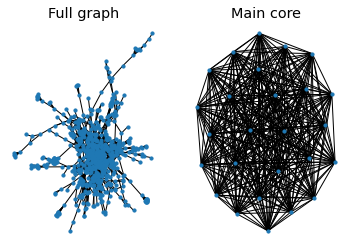
\includegraphics[width=.4\linewidth]{PPIN_fig7}
  \caption{Main core}
  \label{fig:PPIN_fig7}
\end{wrapfigure}

Finally, we explored the main core of each graph. Any complete graph is a core and every graph has a core. The main core is the core with the largest degree. That is, the main core is the largest maximal clique within each network. As a network statistic we considered how many edges each main core has. We expect that the larger the main core of a network, the more resilient it will be to our simulated network failure algorithm. Please see figure 2. Here you can see that the main core of the network shown in the beginning of this paper is a 26-clique with 325 edges. Note that a complete graph of $n$ vertices has $\tfrac{n(n-1)}{2}$ edges.

\subsection{Models}
With network statistics we measure topological stability of PPINs, intending to identify a subset of key network statistics that suffice as significant predictors of the evolutionary time of a species. The question is, which among these network statistics has the most influence on the response variable? With many more variables than data points, we must be careful about overfitting our model to the training data; many machine learning algorithms would produce models that suffer from poor generalization. Moreover, these network statistics are highly correlated with each other, which presents an added challenge, particularly for linear regression models. Consequently, we need to leverage models that afford feature selection. We chose two supervised learning models: LASSO regression and Random Forest regression.

\begin{wrapfigure}{l}[0pt]{0pt}
\centering
  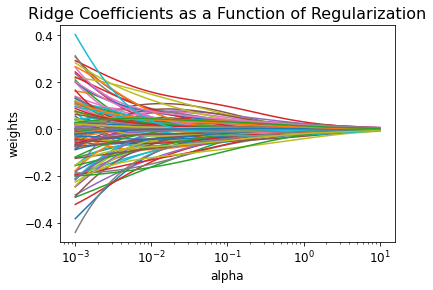
\includegraphics[width=.4\linewidth]{PPIN_fig4}
  \caption{Ridge Tuning}
  \label{fig:PPIN_fig4}
\end{wrapfigure}

The Ridge method regularizes model parameters by shrinking regression coefficients, using the L2 norm (penalty as the sum of squared coefficients). This should reduce the impact of multicollinearity among network statistics while producing interpretable results. We select features assuming that a smaller magnitude regularized coefficients implies lower relevance. We tuned the penalty term of the Ridge regression using \textit{RidgeCV}. Please see figure 3 for a plot of the Ridge coefficients as a function of the regularization penalty. We found that the optimal regularization penalty was $\text{alpha} = 5$.

\clearpage
Random forests build a collection of de-correlated decision trees, by randomly choosing only $m$ predictors from the full set of predictors when performing a split, the split is only allowed to use one of those $m$ predictors. Finally, the average of the resulting trees is taken. In random forest regression, features are selected that improve the variance reduction. That is, correlation between trees is reduced without increasing the variance too much. To tune the hyperparameters for this model we performed an exhaustive search using \textit{GridSearchCV} from Scikit-learn. We tuned the number of estimators, max depth, and max number of features. 

\section{Results}
In figure 4, see that the network statistics with the most influence on the evolutionary time of each species for the Ridge model were average degree centrality, total network density, LCSG density, LCSG algebraic connectivity, modularity, and a handful of the larger number of k-stars variables. The sign of coefficients tells you if the network statistic is positively or negatively related to the response, evolutionary time. See that all of the listed significant statistics are positively related to evolutionary time.
\begin{wrapfigure}{r}{0.5\textwidth}
  \vspace{-20pt}
  \begin{center}
    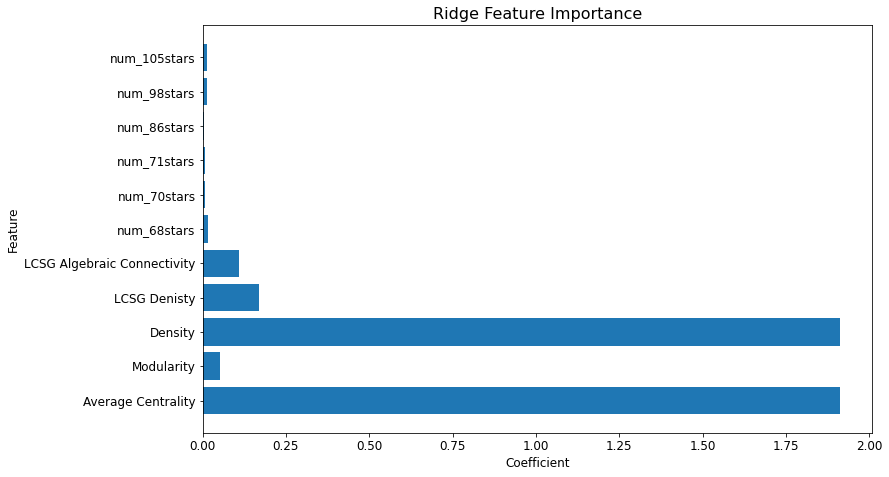
\includegraphics[width=0.548\textwidth]{PPIN_fig3}
  \end{center}
  \vspace{-20pt}
  \caption{Ridge Feature Selection}
  \vspace{-10pt}
\end{wrapfigure}
\indent As the total network density and LCSG density increase, the number of actual connections in a network approaches the number of potential connections. That is, stability increases--making the network more resilient to failure or breakage. Recall that network resilience is the measure of how quickly a network breaks down as nodes are randomly removed and it has been shown that networks with low network resilience also have a low evolutionary time. When a network is highly connected, though not necessarily fully connected, it has higher resilience. In this same way, we can expect average degree centrality and modularity to be positively related to network resilience and evolutionary time.

The numerically second smallest eigenvalue of the Laplacian matrix of a graph is known as the algebraic connectivity of the graph. This eigenvalue is greater than 0 only if the graph is connected. For this reason, we only find algebraic connectivity of the LCSG. The magnitude of this value reflects how well connected the overall graph is and it is always bounded above by node connectivity. The mean squared training error for the Ridge model was 0.01 and the mean squared test error was 0.126. 

The random forest regression model was consistent with the results from above, please see the important variables for this model (See Figure 5). Arguably, the network statistics with the most influence on the evolutionary time of each species for this model were modularity, clique count, LCSG modularity, average centrality, clique-size mean, density, and number of other k-stars statistics.

\begin{wrapfigure}{l}{0.5\textwidth}
  \vspace{-20pt}
  \begin{center}
    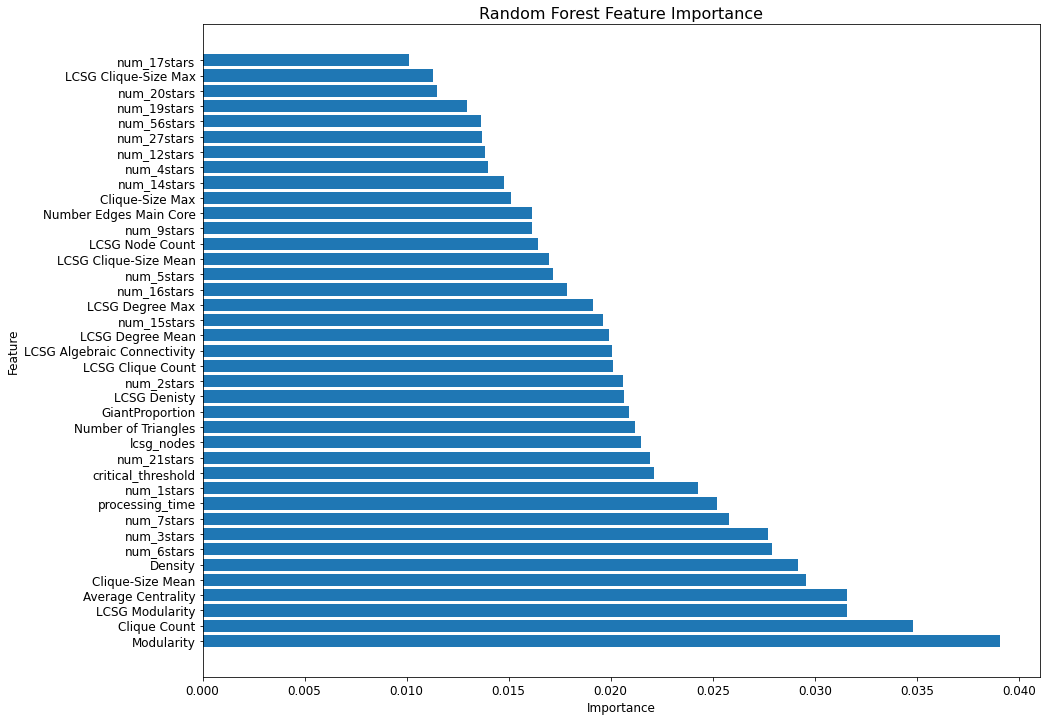
\includegraphics[width=0.5\textwidth]{PPIN_fig2}
  \end{center}
  \vspace{-20pt}
  \caption{Random Forest Feature Selection}
  \vspace{-10pt}
\end{wrapfigure}

The LCSG clique-size mean denotes the average size of a maximal clique within the LCSG. If this number is large, we expect the stability of this network to be strong (higher network resilience). \textbf{Clique Count} (the total number of maximal cliques in the network) has a similar interpretation.

The random forest regression model indicates the critical threshold, processing time, and number of edges in the main core are significant predictors. The mean squared training error for the random forest regression model was 0.005 and the mean squared rest error was 0.028.
\newline

\section{Conclusion}
There are many possible confounders to consider along with our preliminary results: investigative biases towards modeling common or popular organisms, network size, and genome size. It seems the network statistics we assessed so far as model inputs do a fair job of describing topological stability. Many of these network statistics have a significant relationship to evolutionary time of a species.
\section{Appendix}
\subsection{Exhaustive Enumeration of Cliques is Memory-bound}
\begin{wrapfigure}{r}{0.5\textwidth}
  \vspace{-20pt}
  \begin{center}
    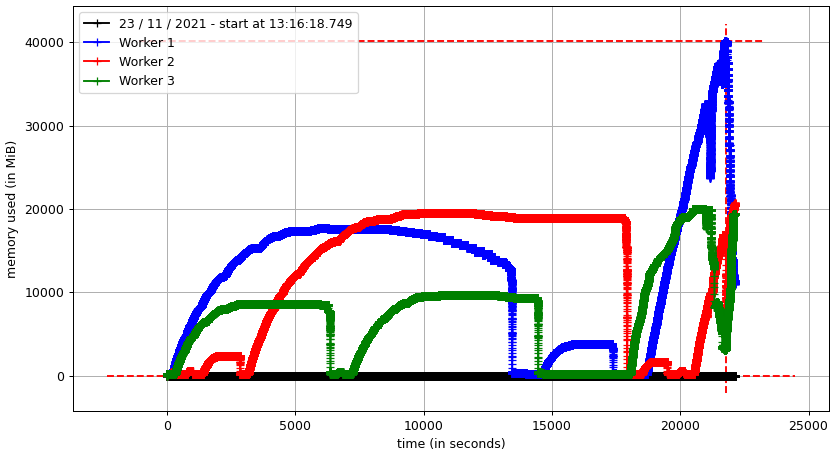
\includegraphics[width=0.48\textwidth]{workers}
  \end{center}
  \vspace{-20pt}
  \caption{$Worker$ memory usage}
  \vspace{-10pt}
\end{wrapfigure}
We tried implementing exhaustive enumeration of \textit{all} cliques (as opposed to \textit{maximal} cliques) but found this to be impractical, as the supporting NetworkX algorithm (\textit{enumerate\_all\_cliques}) is memory-bound. We tested this limitation via execution with 64GB of RAM and 3 $Worker$ processes; execution failed with a $MemoryError$ after $\sim8$ hours of processing, when one of a workers attempted to allocate additional memory beyond available capacity (see Figure 6).
\subsection{K-Stars Algorithm}
Below is pseudocode for how we constructed the data frame of stars counts for each network.
\begin{algorithm}
\caption{Get Stars Algorithm}\label{alg:cap}
\begin{algorithmic}
\State $\text{LCSG } \gets \text{ giant component for undirected network}$
\State $\text{A } \gets \text{ convert LCSG to adjacency matrix}$
\State $\text{d } \gets \text{ sum row elements of A}$
\State $\text{values, counts } \gets \text{ find unique elements and counts for each}$
\State $\text{stars } \gets \text{ pandas DataFrame of counts with index names being values}$
\end{algorithmic}
\end{algorithm}
\begin{table}[H]
\centering
\caption{Count K-Stars Data Frame}
\begin{tabular}{lrrrrrr}
\toprule
Species\_ID &  882   &  883   &  36870 &  52598 &  56780 & $\cdots$\\
\midrule
num\_1stars &  109.0 &   39.0 &   22.0 &   17.0 &   26.0 & $\cdots$\\
num\_2stars &  105.0 &   57.0 &   54.0 &   30.0 &   70.0 & $\cdots$\\
num\_3stars &   65.0 &   63.0 &   31.0 &   20.0 &   53.0 & $\cdots$\\
$\vdots$ &   $\vdots$ &   $\vdots$ &   $\vdots$ &    $\vdots$ &   $\vdots$ & $\ddots$\\
\bottomrule
\end{tabular}
\end{table}

\subsection{Predictors Using NetworkX}
\begin{table}[H]
\centering
\caption{Predictors Using NetworkX Data Frame}
\begin{tabular}{lrrrrrr}
\toprule
Species\_ID &      882   &      883   &    36870 &    52598 &      56780 & $\cdots$ \\
\midrule
Average Centrality          &      0.007 &      0.011 &    0.017 &    0.008 &      0.011 & $\cdots$\\
Number of Triangles         &  12883.000 &  12192.000 &  695.000 &  339.000 &  11755.000 & $\cdots$\\
Modularity                  &      0.710 &      0.730 &    0.695 &    0.796 &      0.640 & $\cdots$\\
Density                     &      0.007 &      0.011 &    0.017 &    0.008 &      0.011 & $\cdots$\\
Clique Count                &   1060.000 &   3580.000 &  209.000 &  823.000 &    547.000 & $\cdots$\\
Clique-Size Max             &     26.000 &     19.000 &   10.000 &    6.000 &     27.000 & $\cdots$\\
Clique-Size Mode            &      2.000 &      5.000 &    2.000 &    2.000 &      2.000 & $\cdots$\\
Clique-Size Mean            &      4.726 &      5.004 &    2.923 &    2.335 &      4.075 & $\cdots$\\
LCSG Clique Count           &    916.000 &    371.000 &  180.000 &  249.000 &    451.000 & $\cdots$\\
LCSG Clique-Size Max        &     26.000 &     19.000 &   10.000 &    5.000 &     27.000 & $\cdots$\\
LCSG Clique-Size Mode       &      2.000 &      2.000 &    2.000 &    2.000 &      2.000 & $\cdots$\\
LCSG Clique-Size Mean       &      5.102 &      4.647 &    3.039 &    2.116 &      4.237 & $\cdots$\\
LCSG Node Count             &    736.000 &    502.000 &  217.000 &  139.000 &    536.000 & $\cdots$\\
LCSG Degree Max             &     60.000 &     58.000 &   27.000 &   11.000 &     66.000 & $\cdots$\\
LCSG Degree Mode            &      1.000 &      3.000 &    2.000 &    2.000 &      2.000 & $\cdots$\\
LCSG Degree Mean            &      9.465 &      9.661 &    5.060 &    4.144 &     10.590 & $\cdots$\\
LCSG Denisty                &      0.013 &      0.019 &    0.023 &    0.030 &      0.020 & $\cdots$\\
LCSG Algebraic Connectivity &      0.016 &      0.011 &    0.008 &    0.017 &      0.018 & $\cdots$\\
LCSG Modularity             &      0.679 &      0.559 &    0.674 &    0.741 &      0.556 & $\cdots$\\
Number Edges Main Core      &    325.000 &    171.000 &   45.000 &   10.000 &    351.000 & $\cdots$\\
Critical Threshold          &    876.500 &    723.900 &  215.500 &  200.500 &    675.100 & $\cdots$\\
Processing Time             &    102.449 &     61.957 &    6.729 &   14.796 &     54.736 & $\cdots$\\
\bottomrule
\end{tabular}
\end{table} \newpage
\begin{thebibliography}{1}
 \bibitem{1} Zitnik, M., Sosič, R., Feldman, M. W., Leskovec, J. (2019). Evolution of resilience in protein interactomes across the tree of life. Proceedings of the National Academy of Sciences, 116(10), 4426-4433. \url{https://doi.org/10.1101/454033}
\bibitem{2} Maddamsetti, R. (2021). Selection maintains protein interactome resilience in the long-term evolution experiment with Escherichia coli. \url{https://doi.org/10.1093/gbe/evab074}
\bibitem{3} Evolution of protein interactomes across the tree of life data. (n.d.). Retrieved from \url{http://snap.stanford.edu/tree-of-life/data.html}
\bibitem{4} Sumit Mukherjee. (2011). Exponential Random graph models. Retrieved from \url{https://artowen.su.domains/courses/319/smukherjee.pdf}
\bibitem{5} Aric A. Hagberg, Daniel A. Schult and Pieter J. Swart, "Exploring network structure, dynamics, and function using NetworkX", in Proceedings of the 7th Python in Science Conference (SciPy2008), Gäel Varoquaux, Travis Vaught, and Jarrod Millman (Eds), (Pasadena, CA USA), pp. 11–15, Aug 2008.
\bibitem{6} Scikit-learn: Machine Learning in Python, Pedregosa et al., JMLR 12, pp. 2825-2830, 2011.
 
\end{thebibliography}

%%%%%%%%%%%%%%%%%%%%%%%%%%%%%%%%%%%%%%%%%%%%%%%%%%%%%%%%%%%%%%%%%%%%%%%%%%%%%
\end{document}
